\partframe{七}{线算子：Wilson 与 't Hooft}

\begin{frame}{线算子}
  \srcp{41} 量子场论里的\emph{线算子}，一般指沿一条嵌入的一维流形 $\gamma$ 修改理论。
  $\gamma$ 可以是闭圈，也可以是端点落在时空边界上的“开”曲线：
  \begin{center}
  \begin{tikzpicture}[scale=0.9,>={Stealth[length=1.5mm]}]
    \draw[thick] (0,0) .. controls (0.8,0.9) and (1.6,-0.7) .. (2.4,0.2);
    \fill (0,0) circle (1.6pt); \fill (2.4,0.2) circle (1.6pt);
    \node[font=\scriptsize,below] at (1.2,-0.55) {$\gamma$（开曲线，端点在边界）};
    \draw[thick] (4.6,0) circle (0.85);
    \node[font=\scriptsize,below] at (4.6,-1.25) {$\gamma'$（闭圈）};
  \end{tikzpicture}
  \end{center}
  在路径积分里，它等价于在 $\gamma$ 的小管状邻域上给定一个边界条件。
\end{frame}

\begin{frame}{Wilson 算子}
  \srcp{42} 最简单的线算子是 Wilson 算子：联络在某个表示 $R$ 下的全纯（holonomy）的迹。
  对闭圈，
  \[
    W_R(\gamma)=\Tr_R\,\mathrm{Hol}_\gamma A
    \;=\;\Tr_R\,P\exp\!\oint_\gamma A .
  \]
  每一个不可约表示 $R$ 给一个 Wilson 算子。
  \begin{beizhu}
  \textbf{批注}\quad 物理上 $W_R$ 描述一个沿 $\gamma$ 运动的“探针”，它在表示 $R$ 下带荷。
  夸克禁闭的判据就是：大圈的 $W_R$ 呈面积律衰减。
  \end{beizhu}
\end{frame}

\begin{frame}{'t Hooft 算子的朴素定义}
  \srcp{43} Wilson 算子用来探夸克禁闭；约 1980 年，这促使 't Hooft 去定义它的电—磁对偶。
  \vspace{0.3em}

  四维中，一维的 $\gamma$ 余维 $3$；围绕它的“链环”是一个二维球面 $S^2$。
  局部不变量是 $S^2$ 上 $G$-丛的拓扑型：
  \[
    \pi_1(G)\;\cong\;\{\text{$S^2$ 上 $G$-丛的拓扑型}\}.
  \]
  \begin{center}
  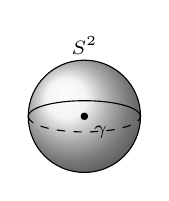
\begin{tikzpicture}[scale=0.62]
    \shade[ball color=black!6] (0,0) circle (1.15);
    \draw (0,0) circle (1.15);
    \draw[dashed] (-1.15,0) arc (180:360:1.15 and 0.32);
    \draw (-1.15,0) arc (180:0:1.15 and 0.32);
    \fill (0,0) circle (2.2pt) node[below right,font=\scriptsize]{$\gamma$};
    \node[font=\scriptsize] at (0,1.45) {$S^2$};
  \end{tikzpicture}
  \end{center}
  但 't Hooft 原来的定义对几何 Langlands 来说不够精确。
\end{frame}

\begin{frame}{Kapustin 的精确化}
  \srcp{44} Kapustin（2005）给了更精确的定义。他的讨论与 't Hooft 不同之处在于：
  他对奇点附近施加更精确的条件，而不只是指定情形的拓扑。
  \vspace{0.4em}

  \srcp{45} 想法是：要求场在 $\gamma$ 附近渐近于杨--米尔斯方程的一个指定的奇异解。
  对余维 $3$ 奇点的局部模型，可以取 $\RR^3$ 原点处的行为。对 $G=U(1)$，荷 $1$ 的
  “狄拉克单极子”解是一个曲率为
  \[
    F_0=\tfrac12\star\dd\frac{1}{|\vec x|}
  \]
  的联络 $A_0$。对任何 $G$（李代数为 $\mathfrak g$），取同态 $\rho:u(1)\to\mathfrak g$，
  并要求在 $\vec x=0$ 附近
  \[
    A\;\sim\;A_\rho:=\rho(A_0).
  \]
\end{frame}

\begin{frame}{型：一个余权}
  \srcp{46} 由于我们只关心 $A_\rho$ 在共轭意义下的类，可以把 $\rho$ 看成到极大环面
  $\mathfrak t$ 的同态：
  \[
    \rho:u(1)\to\mathfrak t ,
  \]
  再模去 Weyl 变换。于是“型”就是一个余权，模 Weyl 群：
  \[
    \{\text{'t Hooft 算子的型}\}\;\cong\;X_*(T)/W .
  \]
  \begin{beizhu}
  \textbf{批注}\quad 对比 Wilson 算子：它由表示 $R$ 标号，也就是由最高权
  $\rho_{\mathrm{el}}:T\to U(1)$ 标号，即 $X^*(T)/W$。
  电与磁，一个是权，一个是余权。这正是第 3 章那张表的物理版本。
  \end{beizhu}
\end{frame}

\begin{frame}{对照表}
  \begin{center}
  \renewcommand{\arraystretch}{1.45}
  \begin{tabular}{@{}lll@{}}
    \toprule
     & Wilson 算子 & 't Hooft 算子 \\
    \midrule
    定义 & 沿 $\gamma$ 的全纯的迹 & 沿 $\gamma$ 的指定奇点 \\
    标号 & $G$ 的表示 $R$ & 同态 $\rho_{\mathrm{mag}}:U(1)\to T$ \\
    群论数据 & 最高权 $\rho_{\mathrm{el}}:T\to U(1)$ & 余权 $\rho_{\mathrm{mag}}:U(1)\to T$ \\
    取值 & $X^*(T)$ & $X_*(T)$ \\
    对偶下 & $G$ 的 Wilson & $\gvee$ 的 't Hooft \\
    \bottomrule
  \end{tabular}
  \end{center}
\end{frame}

\begin{frame}{Montonen--Olive 下的交换}
  \srcp{48} 在规范群为 $G$ 与 $\gvee$ 的两个理论之间的 Montonen--Olive 对偶里，
  $G$ 的 Wilson 算子对应于 $\gvee$ 的 't Hooft 算子，反之亦然。依据是自然对应
  \[
    \rho:T\to U(1)
    \qquad\longleftrightarrow\qquad
    \rho^{\vee}:U(1)\to\Tvee
  \]
  以及 $G$ 与 $\gvee$ 有同一个 Weyl 群。
  \vspace{0.4em}

  这与 1977 年 GNO 的观察是同一件事；区别在于：改用线算子表述之后，
  不必再\textbf{调用希格斯机制}。
  \begin{beizhu}
  \textbf{批注}\quad 这正是 Witten 在 1977 年对 GNO 的不满所在：电与磁的匹配只在
  希格斯化之后才成立，而“根本性的陈述不应依赖希格斯化”。线算子的语言把它修好了。
  \end{beizhu}
\end{frame}

\begin{frame}{从粒子到算子：为什么要换语言}
  \begin{itemize}
    \item 粒子图像：磁荷 $\pi_1(G)$ 只在 $G$ 被破缺到 $T$ 之后才定义。
    \item 算子图像：'t Hooft 算子的型是一个余权，不依赖任何真空的选择。
    \item 好处：对偶成为关于\emph{算子}的陈述，可以在任意耦合下陈述与检验。
  \end{itemize}
  \vspace{0.5em}
  于是“GNO 的磁规范群 = Langlands 对偶群”从一个关于破缺相的事故，
  变成一个关于理论的\emph{结构性}事实。
\end{frame}

\partframe{八}{合流：$\RR\times C$ 上的 Bogomolny 方程}

\begin{frame}{与几何 Hecke 的关系}
  \srcp{49} 这一切与几何 Hecke 修改有什么关系？这里要考虑 Bogomolny 方程——
  它大致支配着四维超对称规范理论的\emph{时间无关}情形。
  \vspace{0.4em}

  在三维中，余维 $3$ 的奇点是一个孤立点：
  \begin{center}
  \begin{tikzpicture}[scale=1.0,>={Stealth[length=1.5mm]}]
    \draw (-1.5,-0.75) -- ++(3.0,0) -- ++(0.55,0.45) -- ++(-3.0,0) -- cycle;
    \draw[->] (0,0.35) -- (0,1.35) node[above,font=\scriptsize]{$\RR^3$};
    \fill[red] (0.9,0.15) circle (2.3pt);
    \node[font=\scriptsize,below right] at (0.95,0.1) {奇点};
  \end{tikzpicture}
  \end{center}
  所以要在 Dirac 型孤立奇点下解 Bogomolny 方程。这类问题最早由 Kronheimer（1986）
  与 Pauly（1990）研究。
\end{frame}

\begin{frame}{$\RR^3=\RR\times\RR^2$ 的两种读法}
  \srcp{50} Atiyah 与 Hitchin 在描述“谱曲线”时，把 $\RR^3$ 分解为 $\RR\times\RR^2$，
  看成 $\RR$ 的\emph{两参数}族。
  \vspace{0.4em}

  这里我们反过来：把 $\RR^3$ 看成 $\RR^2$ 的\emph{一参数}族。而且可以把 $\RR^2$
  换成任意 Riemann 面 $C$。所以我们研究 $\RR\times C$ 上的 Bogomolny 方程，
  把它看成 $C$ 的一参数族，用实变量 $y$ 参数化 $\RR$：
  \begin{center}
  \begin{tikzpicture}[scale=0.95,>={Stealth[length=1.5mm]}]
    \draw (0,0) ellipse (0.55 and 1.15);
    \draw (3.2,0) ellipse (0.55 and 1.15);
    \draw (0,1.15) -- (3.2,1.15);
    \draw (0,-1.15) -- (3.2,-1.15);
    \draw[dashed] (0.55,0) -- (2.65,0);
    \node[font=\scriptsize] at (-1.0,0) {$C$};
    \node[font=\scriptsize] at (2.65,0.15) {$y$};
    \draw[->] (3.5,0) -- (4.1,0);
  \end{tikzpicture}
  \end{center}
  轴向是 $\RR$，每个横截面都是同一条 Riemann 面 $C$。
\end{frame}

\begin{frame}{Atiyah--Bott：全纯结构与 $y$ 无关}
  \srcp{51} 如 Atiyah 与 Bott 所解释的，$G$-丛 $E\to C$ 上的任何联络 $A$ 都决定一个
  全纯 $G_\CC$-丛 $E_\CC$：只需取 $A$ 的 $(0,1)$ 部分，用它来定义 $E$ 的复化上的全纯结构。
  \vspace{0.3em}

  因此 $C\times\RR$ 上的任何规范场 $A$ 都决定一族全纯丛 $E_y\to C$，$y\in\RR$。
  如果 $A$ 满足 Bogomolny 方程
  \[
    F=\star\dd_A\phi ,
  \]
  那么 $E_y$ 作为 $C$ 上的全纯丛，就\textbf{典范地}与 $y$ 无关。这是因为 Bogomolny
  方程的三个实分量中有两个可以写成
  \[
    0=\Bigl[\frac{D}{Dy}+i\phi,\;\frac{D}{D\bar z}\Bigr].
  \]
  第三个方程可以看成一个矩映射条件，类似 Atiyah 与 Bott 在讨论二维杨--米尔斯时所说的。
\end{frame}

\begin{frame}{跨过 $y_0$：一次 Hecke 修改}
  \srcp{52} 现在假设在某个点 $p\times y_0\in C\times\RR$ 处有一个 't Hooft/狄拉克奇点：
  \begin{center}
  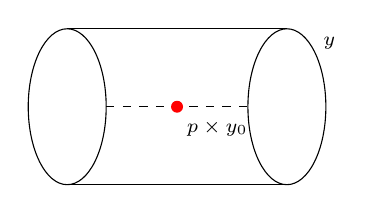
\begin{tikzpicture}[scale=0.9]
    \draw (0,0) ellipse (0.55 and 1.1);
    \draw (3.1,0) ellipse (0.55 and 1.1);
    \draw (0,1.1) -- (3.1,1.1);
    \draw (0,-1.1) -- (3.1,-1.1);
    \draw[dashed] (0.55,0) -- (2.55,0);
    \fill[red] (1.55,0) circle (2.4pt);
    \node[font=\scriptsize,below right] at (1.55,-0.05) {$p\times y_0$};
    \node[font=\scriptsize] at (3.7,0.9) {$y$};
  \end{tikzpicture}
  \end{center}
  那么 $E_y$ 除了 $y=y_0$ 外仍然典范地不依赖 $y$。即使跨过 $y=y_0$，只要把 $E_y$
  限制到 $C\setminus p$ 上，它仍然典范地不依赖 $y$。
  \vspace{0.3em}

  换句话说，在 $y=y_0$ 处发生的事情是：从 $E_y$ 在点 $p$ 作一次 \textbf{Hecke 修改}。
\end{frame}

\begin{frame}{型由奇点决定，对偶给出表示}
  Hecke 修改的“型”由那个特定的 't Hooft/狄拉克奇点决定，而它联系着
  $\rho:U(1)\to T$。
  \vspace{0.4em}

  电—磁对偶把它联系到某个
  \[
    \rho^{\vee}:\Tvee\to U(1),
  \]
  从而联系到对偶群的表示。几何 Hecke 修改与对偶群表示之间的这个关系，
  正是几何 Langlands 对应所断言的那个关系。
  \vspace{0.4em}
  \begin{beizhu}
  \textbf{批注}\quad 现在把三件事对齐：'t Hooft 奇点的型 $=$ 余权 $=$ Hecke 修改的型
  $=$ 对偶群的表示。物理的电磁对偶，恰好把最后一个等号的两端连了起来。
  \end{beizhu}
\end{frame}

\begin{frame}{两个模空间重合}
  \srcp{53} Bogomolny 方程解的模空间，与代数几何里定义的 Hecke 修改的模空间是重合的。
  这一点可以从“第三个”Bogomolny 方程的“矩映射”解释得出。
  \vspace{0.6em}

  \begin{center}
  \begin{tikzpicture}[>={Stealth[length=2mm]},node distance=1.5cm]
    \node[draw,rounded corners,inner sep=7pt,align=center] (a)
      {Bogomolny 解\\（模规范变换）};
    \node[draw,rounded corners,inner sep=7pt,align=center,right=2.6cm of a] (b)
      {Hecke 修改\\（代数几何）};
    \node[font=\scriptsize,below=0.55cm of a] (x) {矩映射条件};
    \node[font=\scriptsize,below=0.55cm of b] (y) {稳定条件};
    \draw[<->,thick] (a) -- node[above,font=\scriptsize]{$\cong$} (b);
  \end{tikzpicture}
  \end{center}
\end{frame}

\begin{frame}{收束}
  \srcp{54} 简而言之，我解释了规范理论对几何 Langlands 对应的解释里的某些主要想法。
  \begin{itemize}
    \item 我试着描述了这个故事如何从 1970 年代 Goddard、Nuyts、Olive 的工作开始，
      以及随后 Montonen 与 Olive 的工作；
    \item 我说了说这个故事如何与数学、物理中的其他发展并行展开；
    \item 我也解释了 Michael Atiyah 在这一过程中所起的影响。
  \end{itemize}
\end{frame}
